% chopout for NIPS 2018 workshop on Compact Deep Neural Networks with industrial applications

\documentclass{article}

    % if you need to pass options to natbib, use, e.g.:
    % \PassOptionsToPackage{numbers, compress}{natbib}
    % before loading nips_2018
        
    % ready for submission
    \usepackage{nips_2018}

    % to compile a preprint version, e.g., for submission to arXiv, add
    % add the [preprint] option:
    % \usepackage[preprint]{nips_2018}
    
    % to compile a camera-ready version, add the [final] option, e.g.:
    % \usepackage[final]{nips_2018}
    
    % to avoid loading the natbib package, add option nonatbib:
    % \usepackage[nonatbib]{nips_2018}

    \usepackage[utf8]{inputenc} % allow utf-8 input
    \usepackage[T1]{fontenc}    % use 8-bit T1 fonts
    \usepackage{hyperref}       % hyperlinks
    \usepackage{url}            % simple URL typesetting
    \usepackage{booktabs}       % professional-quality tables
    \usepackage{amsfonts}       % blackboard math symbols
    \usepackage{nicefrac}       % compact symbols for 1/2, etc.
    \usepackage{microtype}      % microtypography
    \usepackage{amsmath}
    \usepackage{amsthm}
    \usepackage{graphicx}
    \usepackage{float}    
    \usepackage{wrapfig}

    \newtheorem{theorem}{Theorem}   
    \newtheorem{lemma}{Lemma} 

    \newcommand{\maximize}{\mathop{\rm maximize}\limits}
    \newcommand{\minimize}{\mathop{\rm minimize}\limits}
    \newcommand{\argmax}{\mathop{\rm arg~max}\limits}
    \newcommand{\argmin}{\mathop{\rm arg~min}\limits}

    
    \title{Chopout: A Simple Way to Train Variable Sized Neural Networks at Once}
 
    % The \author macro works with any number of authors. There are two
    % commands used to separate the names and addresses of multiple
    % authors: \And and \AND.
    %
    % Using \And between authors leaves it to LaTeX to determine where to
    % break the lines. Using \AND forces a line break at that point. So,
    % if LaTeX puts 3 of 4 authors names on the first line, and the last
    % on the second line, try using \AND instead of \And before the third
    % author name.
    
    \author{
      Tatsuya Shirakawa \\
      ABEJA, Inc. \\
      \texttt{tatsuya@abejainc.com}
      %% examples of more authors
      %% \And
      %% Coauthor \\
      %% Affiliation \\
      %% Address \\
      %% \texttt{email} \\
      %% \AND
      %% Coauthor \\
      %% Affiliation \\
      %% Address \\
      %% \texttt{email} \\
      %% \And
      %% Coauthor \\
      %% Affiliation \\
      %% Address \\
      %% \texttt{email} \\
      %% \And
      %% Coauthor \\
      %% Affiliation \\
      %% Address \\
      %% \texttt{email} \\
    }
    
    \begin{document}
    % \nipsfinalcopy is no longer used
    
    \maketitle
    
    \begin{abstract}
      Large deep neural networks require huge memory to run and their running speed is sometimes too slow for real applications. Therefore network size reduction with keeping accuracy is crucial for practical applications. We present a novel neural network operator, \textit{chopout}, with which neural networks are trained, even in a single training process, so as to truncated sub-networks perform as well as possible. \textit{Chopout} is easy to implement and integrate into most type of existing neural networks. Furthermore it enables to reduce size of networks and latent representations even after training just by truncating layers. We show its effectiveness through several experiments.
    \end{abstract}
    
    % =========================================================
    \section{Introduction}
    % =========================================================
    
    Deep neural networks are crucial building blocks for current artificial intelligence (AI)  because of their outstanding performance in accuracy and ease of use. However, such deep neural networks sometimes run too slow and consume too much memories and, therefore, neural networks with less parameters are preferable for applications.
    
    For this end, various parameter size reduction techniques are developed. They includes 
    (1) pruning techniques which aim to prune weights, channels or layers of neural networks (\citet{han2015deep, aghasi2017nettrim, dong2017learning, molchanov2016pruning, li2017pruning, luo2017thinet, ye2018rethinking, liu2017learning, he2017channel}), 
    (2) quantization techniques which aim to quantize weights of neural networks into $\{+1, -1\}$ or lower precision floating points (e.g. fp16) (\citet{han2015learning, courbariaux2015binaryconnect, rastegari2016xnor, zhou2016dorefa, zhu2016trained,  wu2016quantized, hubara2017quantized}), 
    (3) decomposition techniques which aim to decompose weights with combinations of smaller components (e.g. SVD) (\citet{denton2014exploiting, jaderberg2014speeding, lebedev2014speeding, yang2015deep, novikov2015tensorizing}), 
    (4) distillation techniques which aim to train smaller neural networks (student networks) to mimic trained larger neural networks (teacher networks) (\citet{hinton2015distilling, mishra2017apprentice, polino2018model}) and 
    (5) techniques which aim to design more compact but accurate neural networks (\citet{iandola2016squeezenet, howard2017mobilenet, sandler2018mobilenetv2, zhang2017shufflenet}).

    These techniques sometimes can achieve remarkable parameter reduction without too much accuracy decrease. However some of them have limitations of network architectures, are hard to implement using modern deep learning frameworks such as TensorFlow (\citet{abadi2016tensorflow}), Pytorch (\citet{paszke2017automatic}), or MxNet (\citet{chen2015mxnet}) or require model specific adaptations.

    In this research, we proposed a novel stochastic operator \textit{chopout} which is similar to \textit{dropout} (\citet{srivastava2014dropout}) but randomly truncate latter dimensions/channels of layers in neural networks, with which deep neural networks are trained so that their truncated sub-networks also perform well. 

    %Our main contribution in this research is as follows:
    %\begin{itemize} 
    %  \item we provide a novel operator \textit{chopout} which performs dynamic network reduction in training and enhance the accuracy of their truncated sub-networks as well as possible,
    %  \item we prove that training linear autoencoders with \textit{chopout} is equivalent to computing sigular value decomposition of data matrix
    %  \item and we run experiments and show that truncated sub networks perform well
    %\end{itemize}
    
    % =========================================================
    \section{Method}
    % =========================================================
    \label{sec:method}
    
    \begin{figure}
    \begin{minipage}{0.33\linewidth}
      \begin{center}
        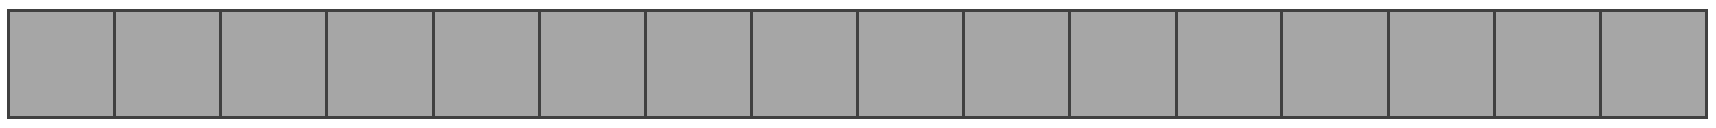
\includegraphics[scale=0.13]{input.png}
        \hspace{1.6cm} (a) input
      \end{center}
    \end{minipage}
    \begin{minipage}{0.33\linewidth}
      \begin{center}
        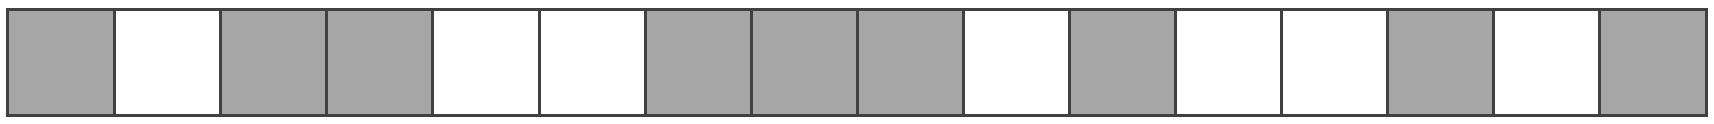
\includegraphics[scale=0.13]{dropout_applied}
        \hspace{1.6cm} (b) dropout
      \end{center}
    \end{minipage}
    \begin{minipage}{0.33\linewidth}
      \begin{center}
        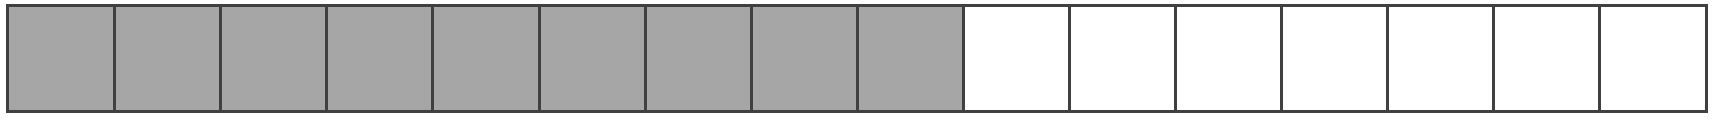
\includegraphics[scale=0.13]{chopout_applied.png}
        \hspace{1.6cm} (c) chopout
      \end{center}
    \end{minipage}    
    \caption{Instead of zeroing out cells in \textit{dropout}, \textit{chopout} truncates random-length latter cells.}
    \label{fig:dropout_and_chopout}
    \end{figure}
    Firstly we define \textit{chopout} for 1-dimensional case.
    At training time, \textit{chopout} is defined as a truncation of random-length latter dimensions of vectors as follows (Figure \ref{fig:dropout_and_chopout}):
    \begin{align}
        m \sim P_m = P(\{0, 1, \cdots, d\}), \ \ 
        \mathbf{x} \leftarrow {proj}_m(\mathbf{x}) := (x_1, x_2, ..., x_m, 0, ..., 0) \nonumber
    \end{align}
    where $P_m = P(\{0, 1, \cdots, d\})$ is aan arbitrary discrete distribution over $\{0, 1, \cdots, d\}$ (e.g. uniform distribution), $\mathbf{x} \in \mathbb{R}^d$ is a vector and ${proj}_m(\cdot)$ is a projection to first $m$-th dimensions. 
    \textit{Chopout}'s behavior is similar to \textit{dropout} but, instead of zeroing out random elements in \textit{dropout}, \textit{chopout} zeros out random latter consecutive elements. In back-propagation, the same latter dimensions of gradients are also zeroed out as well
    \begin{align}
        \mathbf{grad} &\leftarrow {proj}_m(\mathbf{grad}) := ({grad}_1, {grad}_2, ..., {grad}_m, 0, ..., 0) \nonumber
    \end{align}    
    where $\mathbf{grad}$ is a gradient and $m$ is the number drawn in the forward pass. 
    %We denote $chopout(\mathbf{x}; P_m)$ or simplty $chopout(\mathbf{x})$ for the above operator.
    
    At test time, \textit{chopout} is defined to behave as a identity function, that is, just pass through the input vector without any modification. This definition of \textit{chopout} in prediction mode is contrastive to that of \textit{dropout} because ,ordinarily, in prediction mode, \textit{dropout} is defined as a scaling operator corresponding to its drop-rate.
    
    Training a fully-connected neural network with applying \textit{chopout} can be interpreted as training randomly sampled sub-networks which are obtained by cuttinng out \textit{former parts} of the original fully-connected neural network with sharing parameters.

    For higher dimensional case, \textit{chopout} can be easily extended as a random truncation of channels.  For example, when applied to a tensor $\mathbf{x} \in \mathbb{R}^{c \times h \times w}$, the forward-propagation of \textit{chopout} is defined as
    \begin{align}
        m \sim P_m = P(\{0, 1, \cdots, c\}), \ \ 
        x_{kij} \leftarrow \begin{cases}
            x_{kij} & (k \leq m) \\
            0 & (otherwise)
            \end{cases} \nonumber
    \end{align}
    where $P(\{0, 1, \cdots, c\}$ is also an arbitrary distribution as well.

    % =========================================================    
    \section{Experiments}
    % =========================================================    
    \label{experiments}
    
    Throughout experiments, we use uniform distributions over $\{1, \cdots, d\}$ for $P_m(\{0, 1, \cdots, d\})$.

    \subsection{Autoencoder}

    \begin{table}
        \caption{Autoencoders used in experiments. L(n) denotes the linear layer with $n$-dimensional output, R denotes the rectified linear unit function and S denotes the sigmoid function. \textit{Chopout} and \textit{dropout} is applied right after applying the encoder.}    
        \centering
        \begin{tabular}{c|c|c}
            dataset & encoder & decoder \\ \hline \hline
            MNIST & L(100)-R-L(100)-R-L(100) & L(100)-R-L(100)-R-L(784)-S
        \end{tabular}
        \label{tab:mnist_ae}
    \end{table}
    
    \begin{figure}
    \begin{minipage}{0.33\linewidth}
      \begin{center}
        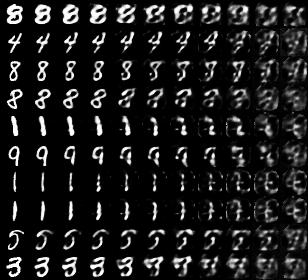
\includegraphics[scale=0.4]{mnist_ae_wo_50.jpg}
        \hspace{1.6cm} (a) normal
      \end{center}
    \end{minipage}
    \begin{minipage}{0.33\linewidth}
      \begin{center}
        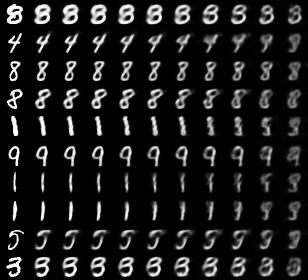
\includegraphics[scale=0.4]{mnist_ae_dropout_50.jpg}
        \hspace{1.6cm} (b) with dropout(p=0.5)
      \end{center}
    \end{minipage}
    \begin{minipage}{0.33\linewidth}
      \begin{center}
        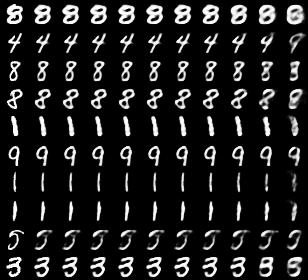
\includegraphics[scale=0.4]{mnist_ae_chopout_50.jpg}
        \hspace{1.6cm} (c) with chopout
      \end{center}
    \end{minipage}    
    \caption{(a) reconstruction of test images by a autoencoder wihout \textit{chopout} and \textit{dropout}, (b) with \textit{dropout} and (c) with \textit{chopout}. 
    In each figure, the left most column represents input images and, from next column to the most right one, each column correspond to the reconstruction results with truncating latter 0, 10, 20, 30, ..., 90 dimensions of hidden layers.}
    \label{fig:mnist_ae}
    \end{figure}
    
    We train autoencoders on MNIST (Table \ref{tab:mnist_ae}, Figure \ref{fig:mnist_ae}). We see that by applying \textit{chopout} on hidden layer of the autoencoder, the reconstruction is kept well even after the hidden layer is truncated.
    
    \subsection{Skip-gram}
    
    \begin{table}[h]
        \caption{top-5 most similar words for learnt 512-dim embeddings. The results of 64-dim embeddings obtained by truncation are also shown.}    
        \centering
        \begin{tabular}{c|c|c|c|c|c}
            ran (512) & ran (64) & news (512) & news (64) & good (512) & good (64) \\ \hline \hline
            stopped & rides & unofficial & openoffice & clever & balanced \\
            stood & stayed & headline & unofficial & strong & queueing \\
            graduated & shot & homepage & overviews & suitable & transparent \\
            struck & sank & portal & bbc & unusually & recursive \\
            shot & fired & online & portal & very & shorthand \\
        \end{tabular}
        \label{tab:skip_gram}
    \end{table}    
    
    We apply \textit{chopout} for embeddings trained through skip-gram models (\citet{mikolov2013efficient, mikolov2013distributed}). We use text8 corpus \footnote{http://mattmahoney.net/dc/text8.zip}. We set the window size to 5 and ignore infrequent words which appear less than 20 times in the corpus. The result (Table \ref{tab:skip_gram}) shows the consistency of embeddings.

    \subsection{Image classification}
    
    \begin{wrapfigure}{r}{75mm}
    \centering
    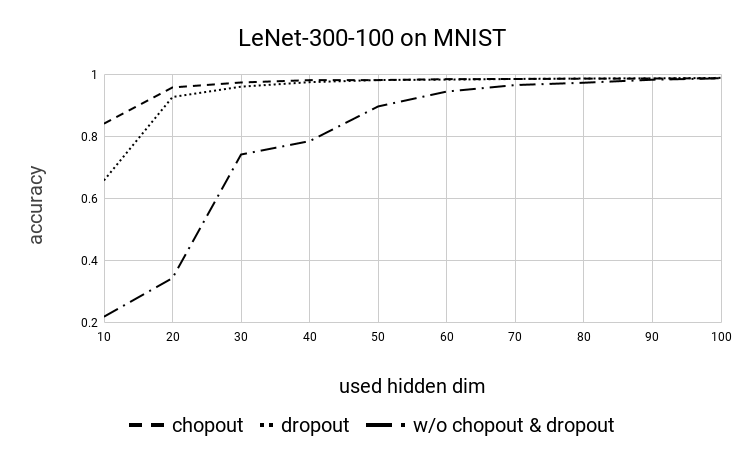
\includegraphics[clip, width=75mm]{lenet-300-100_mnist.png}
    \caption{chopout/dropout is applied in each intermediate layer.}
    \label{fig:lenet-300-100_mnist}
    \end{wrapfigure}
    
    We train LeNet-300-100 (\citet{lecun1998gradient}) on MNIST with and without \textit{chopout} and \textit{dropout} in each intermediate layer (Figure \ref{fig:lenet-300-100_mnist}). This is a very initial experiment but the result shows training with \textit{chopout} enhance the robustness of networks against pruning.
    
    \section{Discussion}
    We introduced a novel and easy stochastic operator \textit{chopout} and showed it gather important information in the former parts of layers. Because the concept of \textit{chopout} is very simple and flexible, there could be broad direction of further research.

    (1) The distribution $P_m(\{0, 1, \cdots, d\})$ should be explored. If we put \textit{chopout}s in every layer of a neural network, then, in training, there could be a layer where drawn $m \sim P_m(\{0, 1, \cdots, d\})$ is very small and it could be bottleneck of the prediction accuracy.
    
    (2) \textit{Chopout} can be used for network pruning. The information-gathering property of \textit{chopout} enables to prune latter dimensions/channels of layers with keeping accuracy but the extent of pruning is still be explored. For this end, reinforcement learning techniques (e.g. bandit algorithms) can be used to detect the appropreate pruning ratio. Combination with weight pruning methods are also interesting as well.

    %\bibliography{references}
    
    %\section*{References}
    
    %\medskip
    
    %\small
        
    \bibliographystyle{plainnat}
    \bibliography{references}
    
    \end{document}